\begin{figure}[!h]
\centering
\resizebox{\columnwidth}{!}{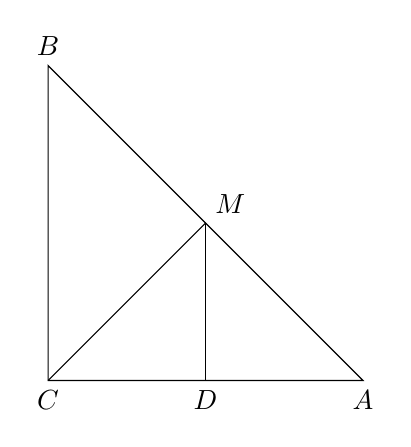
\begin{tikzpicture}
\coordinate (B) at (0,4);
\coordinate (A) at (4,0);
\coordinate (C) at (0,0);
\coordinate (D) at (2,0);
\coordinate (M) at (2,2);
\draw (A)node[below]{$A$}--(B)node[above]{$B$}--(C)node[below]{$C$}--cycle;
\draw(M)node[above right]{$M$}--(D)node[below]{$D$};
\draw(M)--(D);
\draw(M)--(C);
\tkzMarkRightAngle(B,C,A)
\tkzMarkRightAngle(A,D,M)
\tkzMarkRightAngle(C,D,M)
\end{tikzpicture}
}
\caption{Right Angled Triangle by Latex-Tikz}
\label{myfig:solutions/1/7}
\end{figure}
In $\triangle{ABC}$, $\vec{M}$ is midpoint of AB and MD is parallel to BC, hence,
\begin{align}
&\vec{M} = \frac{\vec{A}+\vec{B}}{2}\label{eq:solutions/1/71}\\
&MD \parallel BC\label{eq:solutions/1/72}
\end{align}
Let $\vec{m_{MD}}$ and $\vec{m_{BC}}$ are direction vectors of MD and BC respectively. Then,
\begin{align}
\vec{m}_{MD} &= \vec{M} - \vec{D} = \frac{\vec{A}+\vec{B}}{2} - \vec{D}\\
\vec{m}_{BC} &= \vec{B} - \vec{C}
\end{align}
Now from \eqref{eq:solutions/1/72} we get,
\begin{align}
\vec{m}_{MD} &= k\vec{m}_{BC}\\
\implies\frac{\vec{A}+\vec{B}}{2} - \vec{D} &= k(\vec{B} - \vec{C})\label{eq:solutions/1/7New1}
\end{align}
Let $\vec{D}$ = $\frac{m\vec{A}+\vec{C}}{m+1}$, then from \eqref{eq:solutions/1/7New1} we get,
\begin{align}
\frac{\vec{A}+\vec{B}}{2} - \frac{m\vec{A}+\vec{C}}{m+1} = k(\vec{B} - \vec{C})
\end{align}
\begin{align}
\implies\brak{\frac{1}{2}-\frac{m}{m+1}}\vec{A}+\brak{\frac{1}{2}-k}\vec{B}+\brak{k-\frac{1}{m+1}}\vec{C} =0
\end{align}
Since $\vec{A}$, $\vec{B}$ and $\vec{C}$ are linearly dependent as they form $\triangle{ABC}$ then 
\begin{align}
\frac{1}{2}-\frac{m}{m+1} &= 0\label{solve1}\\
\frac{1}{2}-k & = 0\label{solve2}\\
k-\frac{1}{m+1} &= 0\label{solve3}
\end{align}
Solving \eqref{solve1}, \eqref{solve2} and \eqref{solve3} we get $k=\frac{1}{2}$ and $m = 1$. Hence, substituting value of $m$ in $\vec{D}$ we get,
\begin{align}
&\vec{D} = \frac{\vec{A}+\vec{C}}{2}\label{eq:solutions/1/73}
\end{align}
Hence Proved.\\
From figure \ref{myfig:solutions/1/7},
\begin{align}
(\vec{M}-\vec{D})(\vec{A}-\vec{D}) &=\brak{\frac{\vec{A}+\vec{B}}{2} - \frac{\vec{A}+\vec{C}}{2}}(\vec{A}-\vec{C})\\
\implies(\vec{M}-\vec{D})(\vec{A}-\vec{D}) &=\frac{1}{2}\brak{\vec{B}-\vec{C}}(\vec{A}-\vec{C})\\
\implies(\vec{M}-\vec{D})(\vec{A}-\vec{D}) &=0\label{eq:solutions/1/74}\quad \because BC\perp AC
\end{align}
From \eqref{eq:solutions/1/74}, it is proved that MD$\perp$AC\\
Again we get,
\begin{align}
\vec{C-M} &= \vec{C - D}+\vec{D - M}\\
\implies\vec{C-M} &= \vec{A - D}+\vec{D - M}\quad\text{[From \eqref{eq:solutions/1/73}]}\\
\implies\vec{C - M} &= \vec{A - M}\label{eq:solutions/1/7Fin1}\\
\implies\vec{C - M} &= \vec{A} - \vec{\frac{\vec{A}+\vec{B}}{2}}\qquad\text{[From \eqref{eq:solutions/1/71}]}\\
\implies\vec{C - M} &= \frac{1}{2}(\vec{A-B})\\
\implies\norm{\vec{C - M}} &= \frac{1}{2}\norm{\vec{A-B}}\label{eq:solutions/1/7Fin2}
\end{align}
Hence from \eqref{eq:solutions/1/7Fin1} and \eqref{eq:solutions/1/7Fin2} proved,\\CM = MA = $\frac{1}{2}$ AB
